\chapter{Dynamic Resource Management Architecture}\label{chapter:dynamic resource}

\section{System Design}

This section illustrates and describes a high level design of the software implemented with the help of protocol sequence diagrams and state machine diagrams. It will help to understand at a high level as to how the system has been designed to support this new approach of invasive computing and how will many of its components in the software hierarchy interact with each other with new protocols or extensions of existing protocols to integrate such an invasive resource management into current batch systems.\\

The following page shows the software architecture of how Invasive Resource Management can be supported with a traditional resource manager and how exactly the new software components will fit in the existing software hierarchy. The \ref{fig:7} relates closely to how SLURM is organized since the intention of this work would be to demonstrate the support for Invasive Computing with the help of SLURM as a resource manager.
\begin{itemize}
\item The top layer is that of the core resource management component which has access to job queues. In this architecture, it will now have access to not only the queue for the legacy(static) jobs but also invasive job queue(jobs submittted to invasic partition that supports invasive computing).
\item In a traditional setup the top layer will perform the task of job scheduling as well. This means that it will select a job(s) from the queue of jobs based on the current state of resources and many other factors to dispatch it to the traditional process manager below in the hierarchy. The process manager then takes the responsibility of launching these jobs on the allocated resources in the partition and managing them for their full lifetime. In case of parallel jobs, it will manage the job in a parallel environment along with facilitating the communication amongst the parallel tasks/processes with the help of a PMI(Process Manager Interface) server. The process manager may also spawn slave daemons on each of the nodes which are a part of the resource allocation for a single job to manage them more effectively.
\item As discussed in the previous chapter, an independent Invasive resource management component by the name "iHypervisor" will be implemented which needs to communicate with a new scheduling component iScheduler and influence the scheduling decisions taken by it. The iHypervisor sits between the top layer and the process manager.
\item A new job scheduler specifically for invasive jobs needs to be integrated into the existing batch system. This is due to the reason that the scheduler for invasive jobs will work in a different manner based on the approach described earlier in comparison to the legacy job scheduler for static jobs. In case of SLURM which has a modular design with several optional plugins, a new plugin by name "iScheduler" will be implemented for SLURM to handle job scheduling specifically for invasic jobs.
\item Communication between iHypervisor and iScheduler will involve the negotiation protocol as explained in the previous chapter but will also include periodic feedbacks being sent by iHypervisor to iScheduler having some useful statistical measures about current state of resources, resource utilization, job throughput etc. that may help influence the decision making of iScheduler. This communication will also additionally support a means to service urgent jobs immediately.
\end{itemize}
\begin{figure}[!htbp]
\centering
%\includegraphics[width=1.0\textwidth, height=185mm]{./figures/"software architecture".pdf}
\includegraphics[width=1.0\textwidth, height=185mm]{./figures/"software architecture".eps}
\caption{Invasive Resource Management Architecture}
\label{fig:7}
\end{figure}
\begin{figure}[h]
\centering
%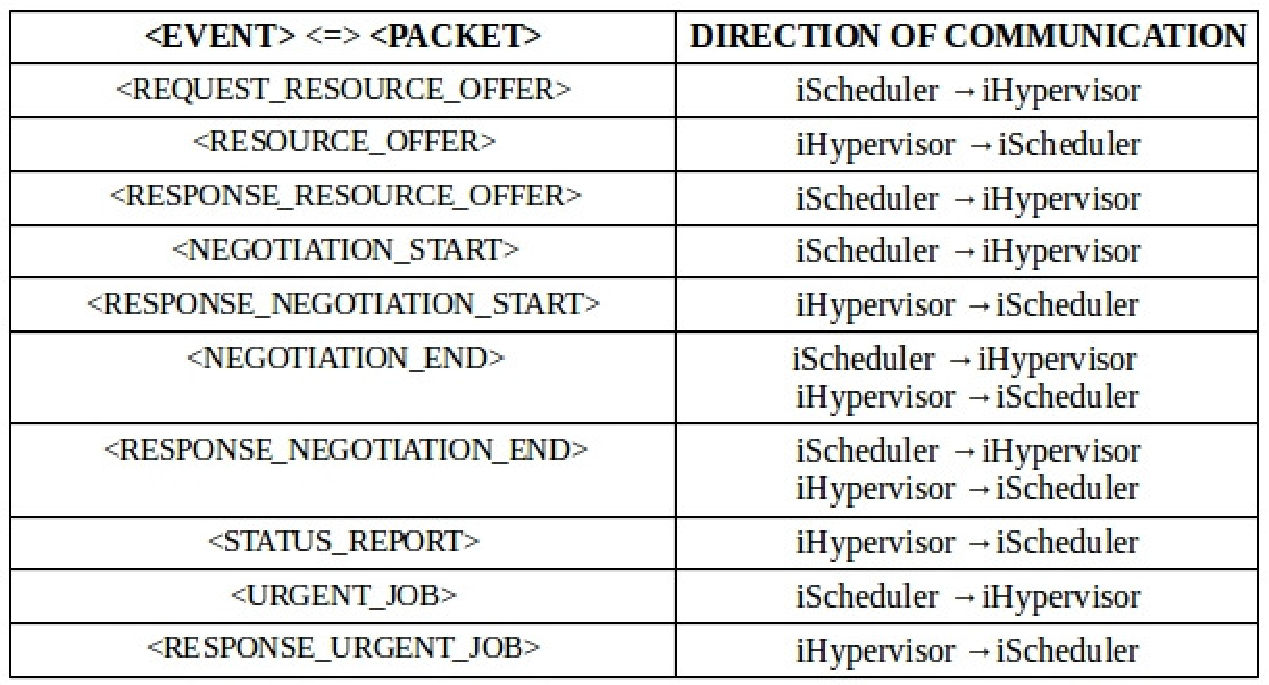
\includegraphics[width=1.0\textwidth, height=80mm]{./figures/table.pdf}
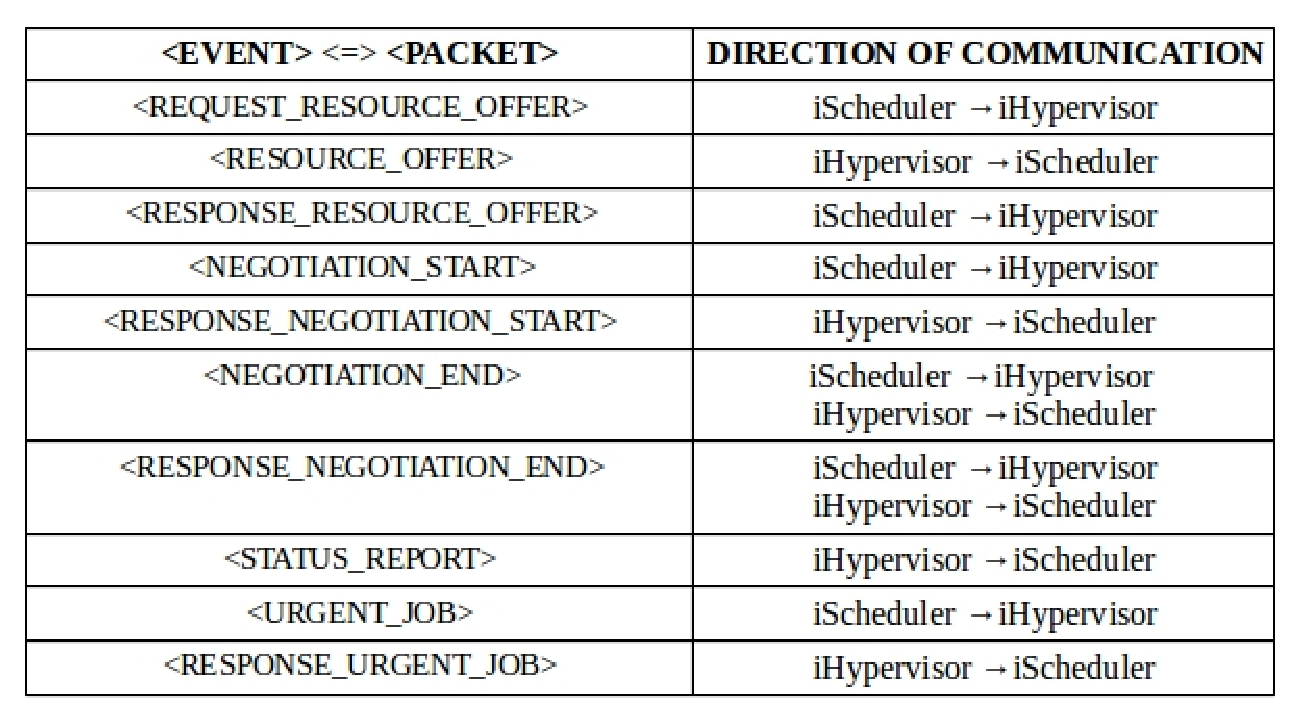
\includegraphics[width=1.0\textwidth, height=80mm]{./figures/table.eps}
\caption{Message Types}
\label{fig:8}
\end{figure}

\textbf{Communication Phases}
\begin{itemize}
\item \textbf{\textit{Protocol Initialization:}} This phase basically establishes the initial environment between the communicating parties (iScheduler and iHypervisor) for proper communication later on. Successful initialization of this phase prepares both the parties to start negotiating based on the negotiation protocol described in the following points. During this protocol initialization various parameters such as protocl version, maximum attempts for negotiation, timer intervals and several others could be exchanged to set up the internal data structures and configuration tables for both the communicating parties. This protocol is a bi-directional communication.
\item \textbf{\textit{Protocol Finalization:}} This phases signals the end of communication between iHypervisor and iScheduler using negotiation protocol. It leads to a safe termination of this communication followed by the release of any internal data structures allocated earlier along with configuration parameters. This results in consistent behaviour of both the communicating parties which can then proceed to safely terminate and exit. This protocol is a bi-directional communication.
\item \textbf{\textit{Negotiation:}} This is the most important phase in this whole approach to support invasive computing as discussed in the previous chapter. It is the phase during which both iHypervisor and iScheduler are negotiating with each other till they reach an agreement. If they do not then they continue till a certain limit to the number of negotiating attempts are reached after which both of them just agree in their final attempt closing the current negotiation. After this a new transaction of negotiation begins.
\item \textbf{\textit{Feedback:}} This concerns the periodic feedback sent by the iHypervisor to the iScheduler containing useful information such as the job states, latest snapshot of the resources in the invasic partition and many other statistical measures not limited to system utilization, job throughput, waiting times of jobs to help and influence the iScheduler in its decision making for scheduling jobs during its future transactions of negotiation. This protocol is a uni-directional communication.
\item \textbf{\textit{Urgent Jobs:}} This protocol concerns the support for urgent jobs. At any given point of time a cluster or supercomputing center may want to support very high priority jobs immediately without any further delay. By introducing support for invasive computing, it makes it all the more feasible to help run these urgent jobs immediately by either shrinking the resources of other jobs or suspending/Killing them.
\end{itemize}

\textbf{\textit{Separation of Concerns: }}In this thesis, The idea of separating the batch and runtime scheduling components of a Job Scheduler is explored. 

\subsection{Batch Scheduler}
Today almost all resource management systems fall into the category of queuing systems. Several queues with different limits on the number of requested resources and the duration exist for the submission of resource requests. Jobs within a queue are ordered according to a scheduling policy, e. g. FCFS (first come, first serve). Queues might be activated only for specific times (e. g. prime time, non prime time, or weekend). The task of a queuing system is to assign free resources to waiting requests. The highest prioritized request is always the queue head. If it is possible to start more than one queue head, further criteria like queue priority or best fit (e. g. leaving less resources idle) are used to select a request. There might also exist a high priority queue whose jobs are preferred at any time. If not enough resources are available to start any of the queue heads, the system waits until enough resources become available. These idle resources may be utilized with less prioritized requests by backfilling mechanisms.
\subsection{Distributed Run Time Scheduler}
\subsection{MPI Process Manager}


\section{Negotiation Protocol}
\subsection{Protocol Sequence Diagrams}
\vspace{-0.15in}
\begin{figure}[!htbp]
%\begin{figure}[H]
\centering
%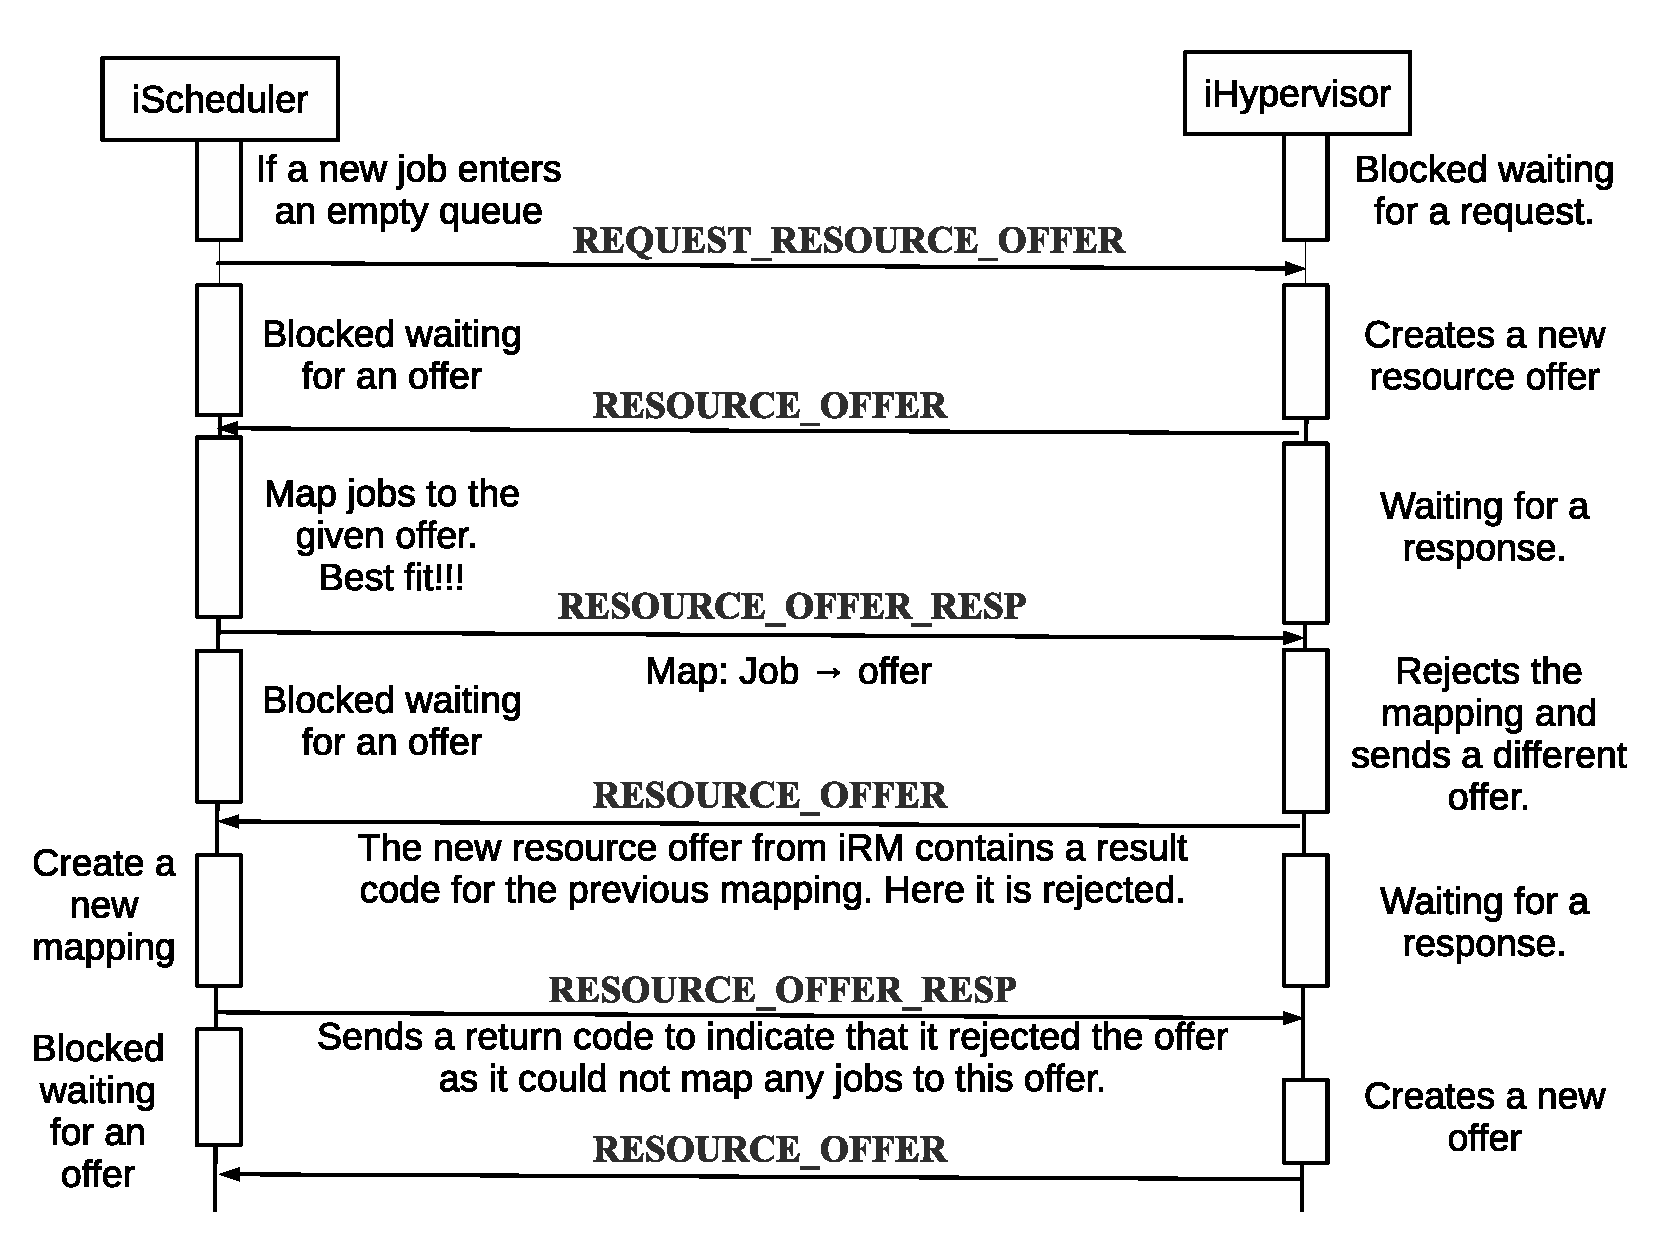
\includegraphics[width=1.0\textwidth, height=100mm]{./figures/figures.pdf}
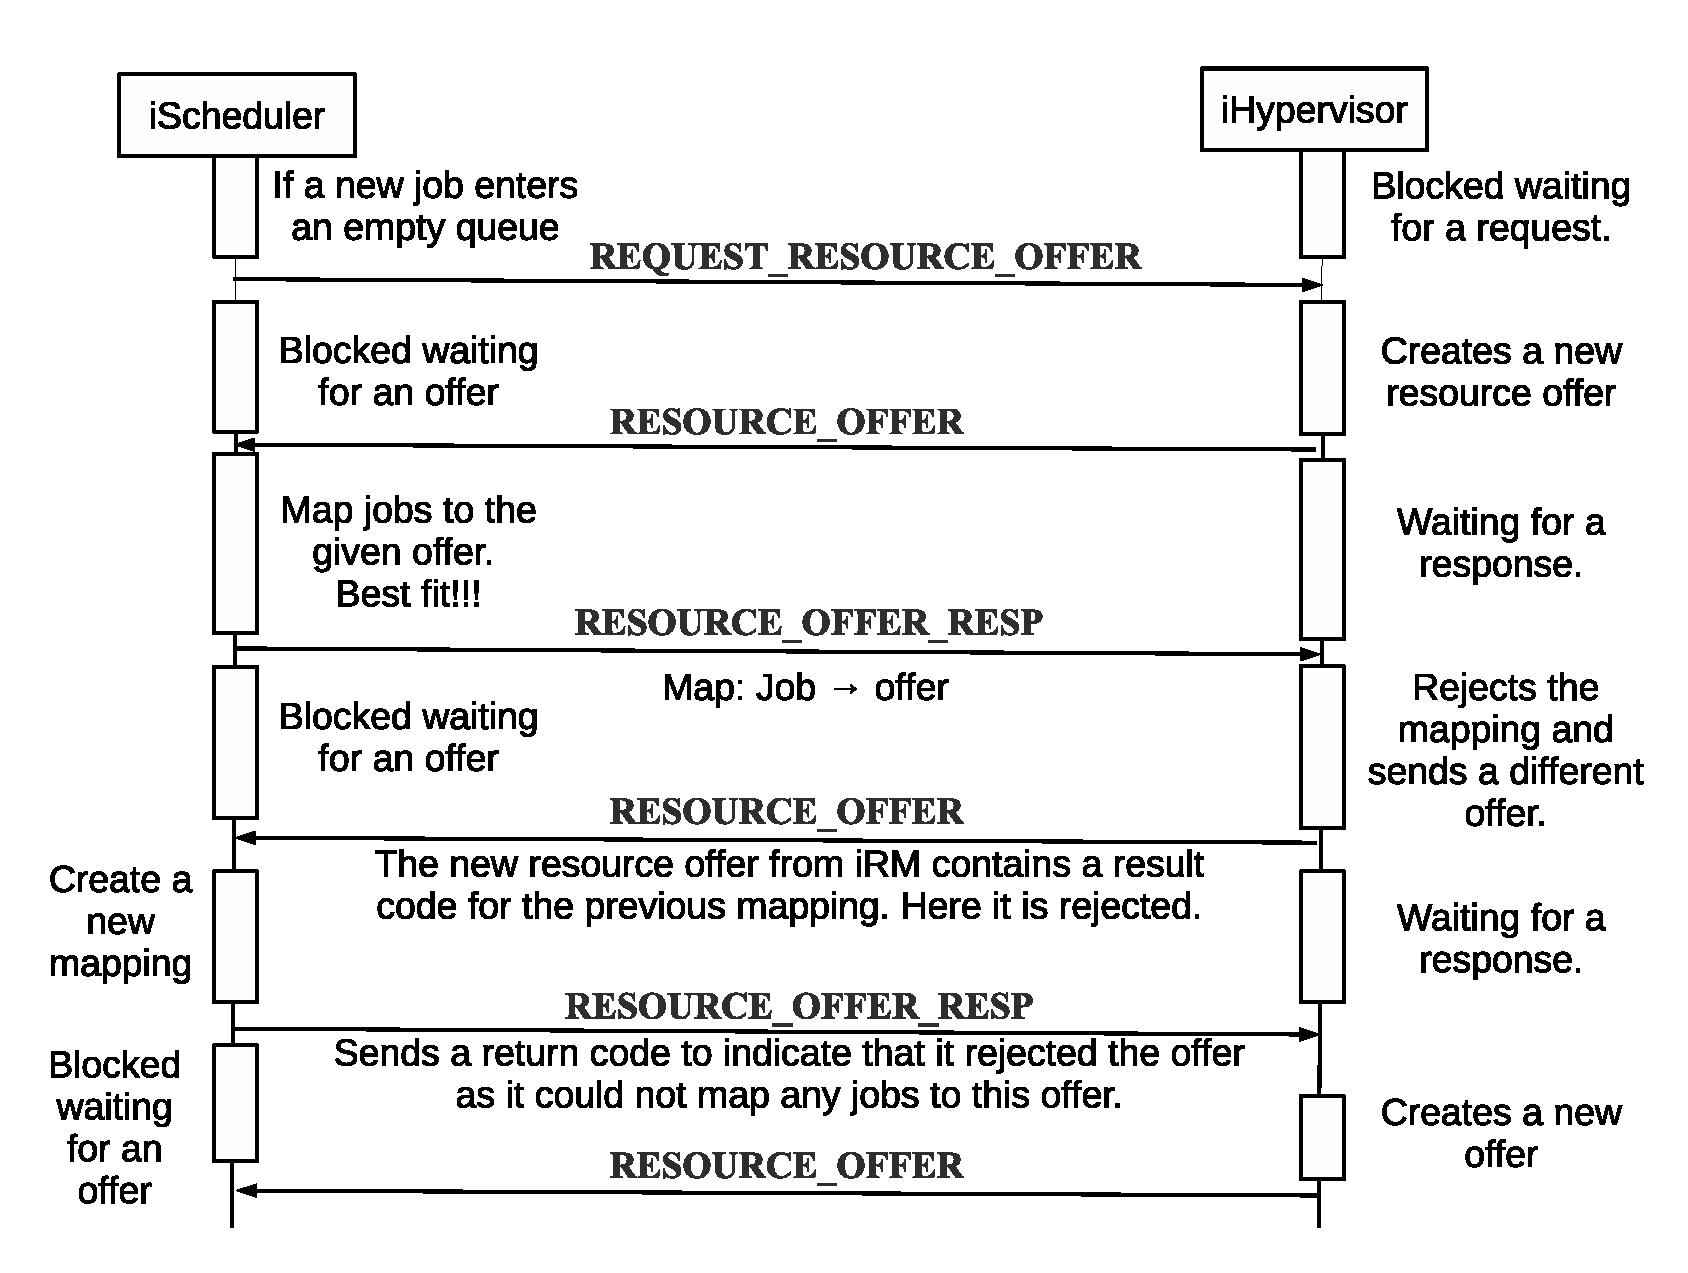
\includegraphics[width=1.0\textwidth, height=100mm]{./figures/figures.eps}
\caption{Scenario 1}
\begin{itemize}
\item Above diagram illustrates a scenario where both iScheduler and iHpervisor are negotiating with each other. The scenario is continued in the next page. \ref{fig:Seq2} illustrates another scenario where negotiations may stop when job queue becomes empty and iHypevisor then will wait for a request from iScheduler for a resource offer that will happen when new jobs arrive.
\item iScheduler makes scheduling decisions at a coarser level of granularity which is nodes whereas iHypervisor does at the granularity of cores and sockets. Both will negotiate with each other till they reach an agreement.
\item It is an event based scheduling which means iScheduler makes a scheduling decision only when it is triggered by receiving a resource offer from iHypervisor. It is only at the start when there are no jobs in the queue and during the operations when the queue may become empty that the iScheduler will have to explicitly send a request message to iHypervisor for a resource offer otherwise at all other times scheduling is event based.
\end{itemize}
\label{fig:Seq1}
\end{figure}
\vspace{-0.25in}
\begin{figure}[!htbp]
\centering
%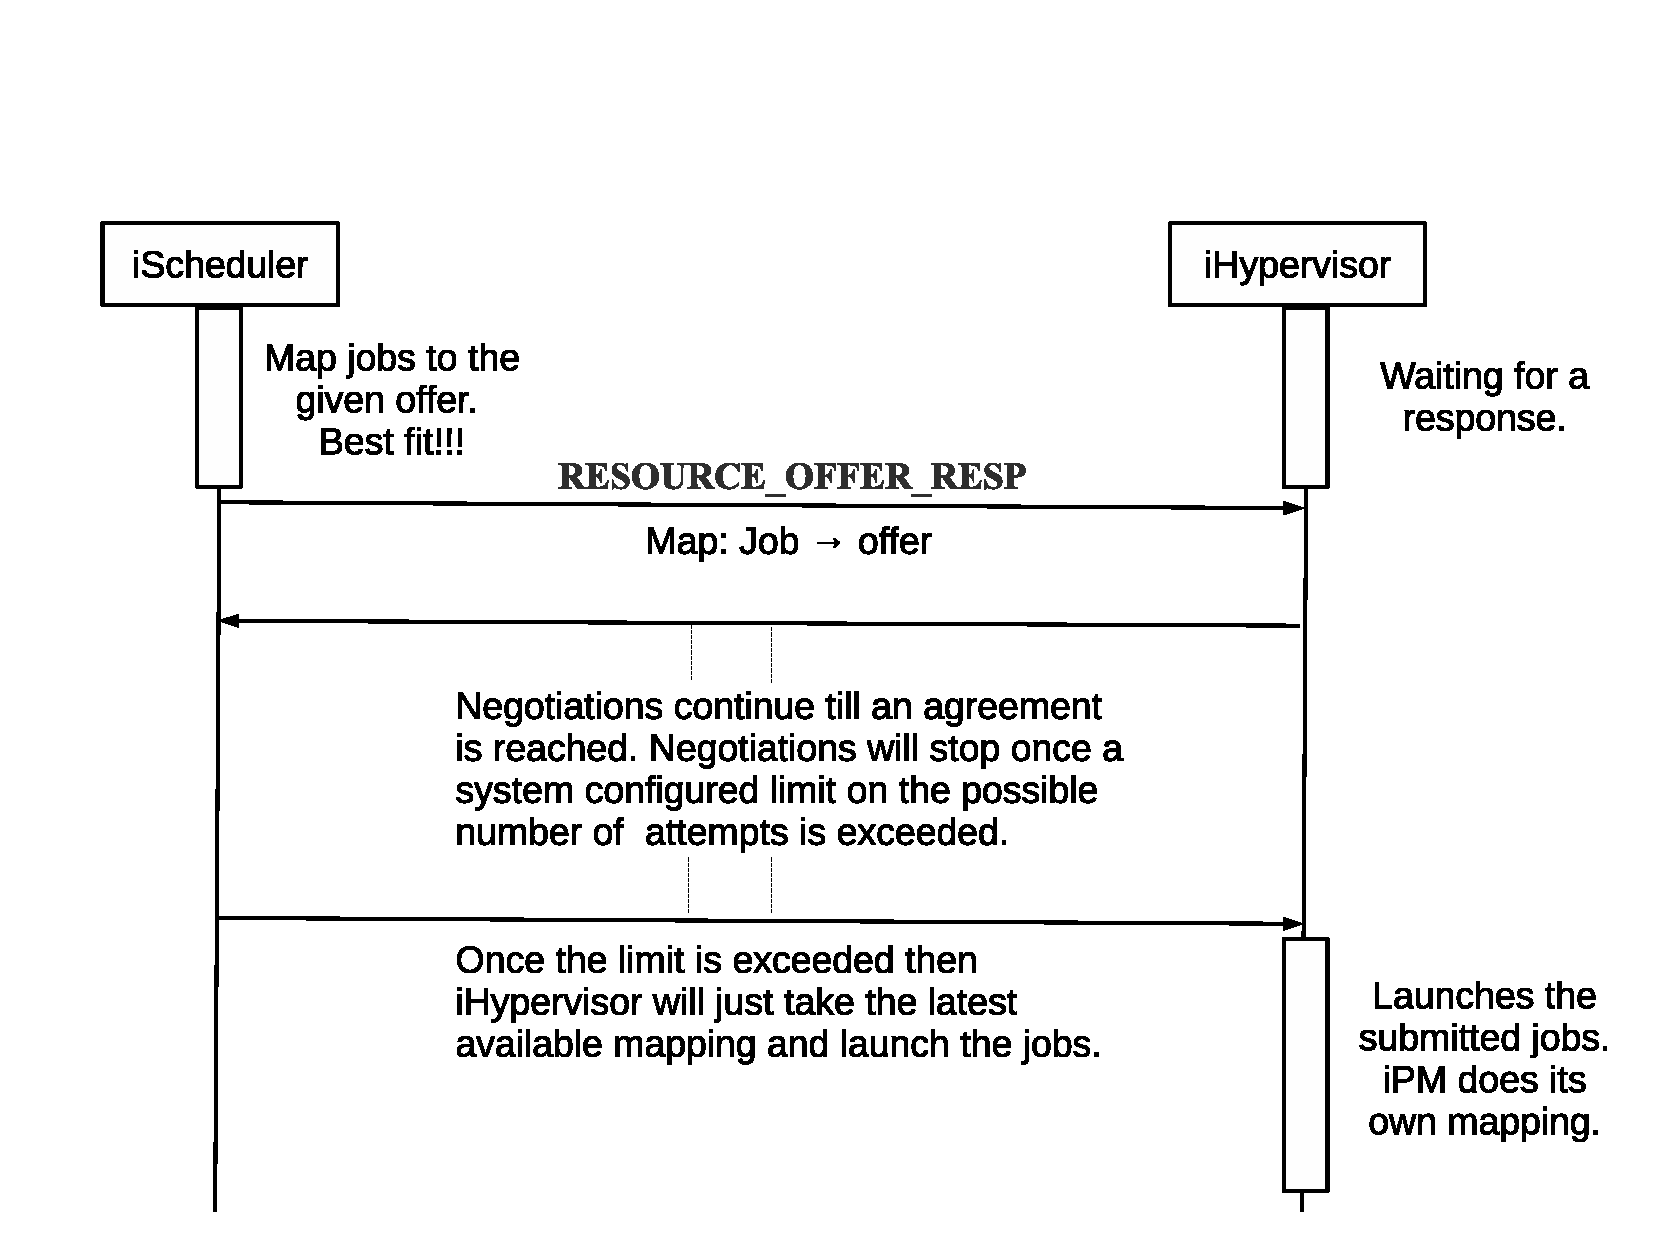
\includegraphics[width=0.9\textwidth, height=100mm]{./figures/figures1.pdf}
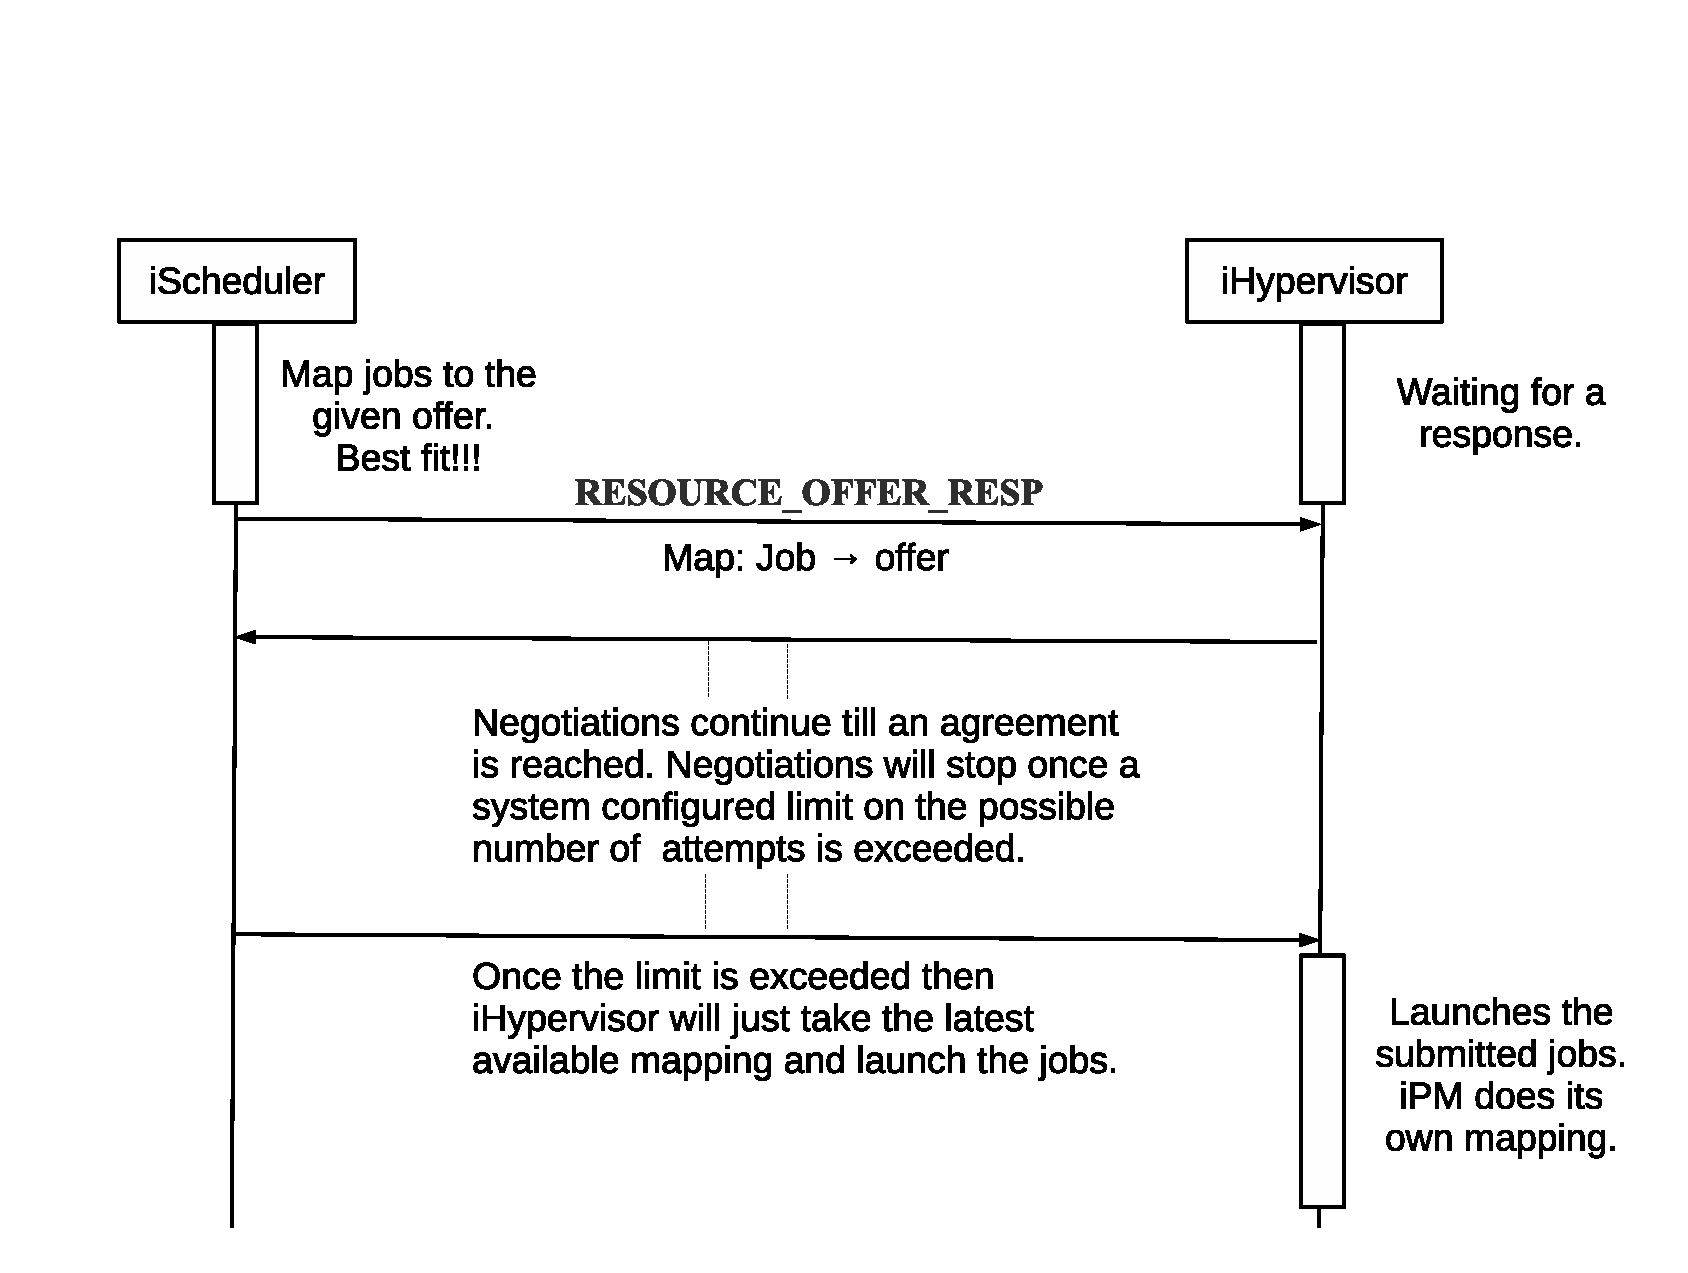
\includegraphics[width=0.9\textwidth, height=100mm]{./figures/figures1.eps}
\caption{Scenario 1 contd.}
\label{fig:Seq1}
\vspace{0.25in}
%\end{figure}
%\begin{figure}[b]
\centering
%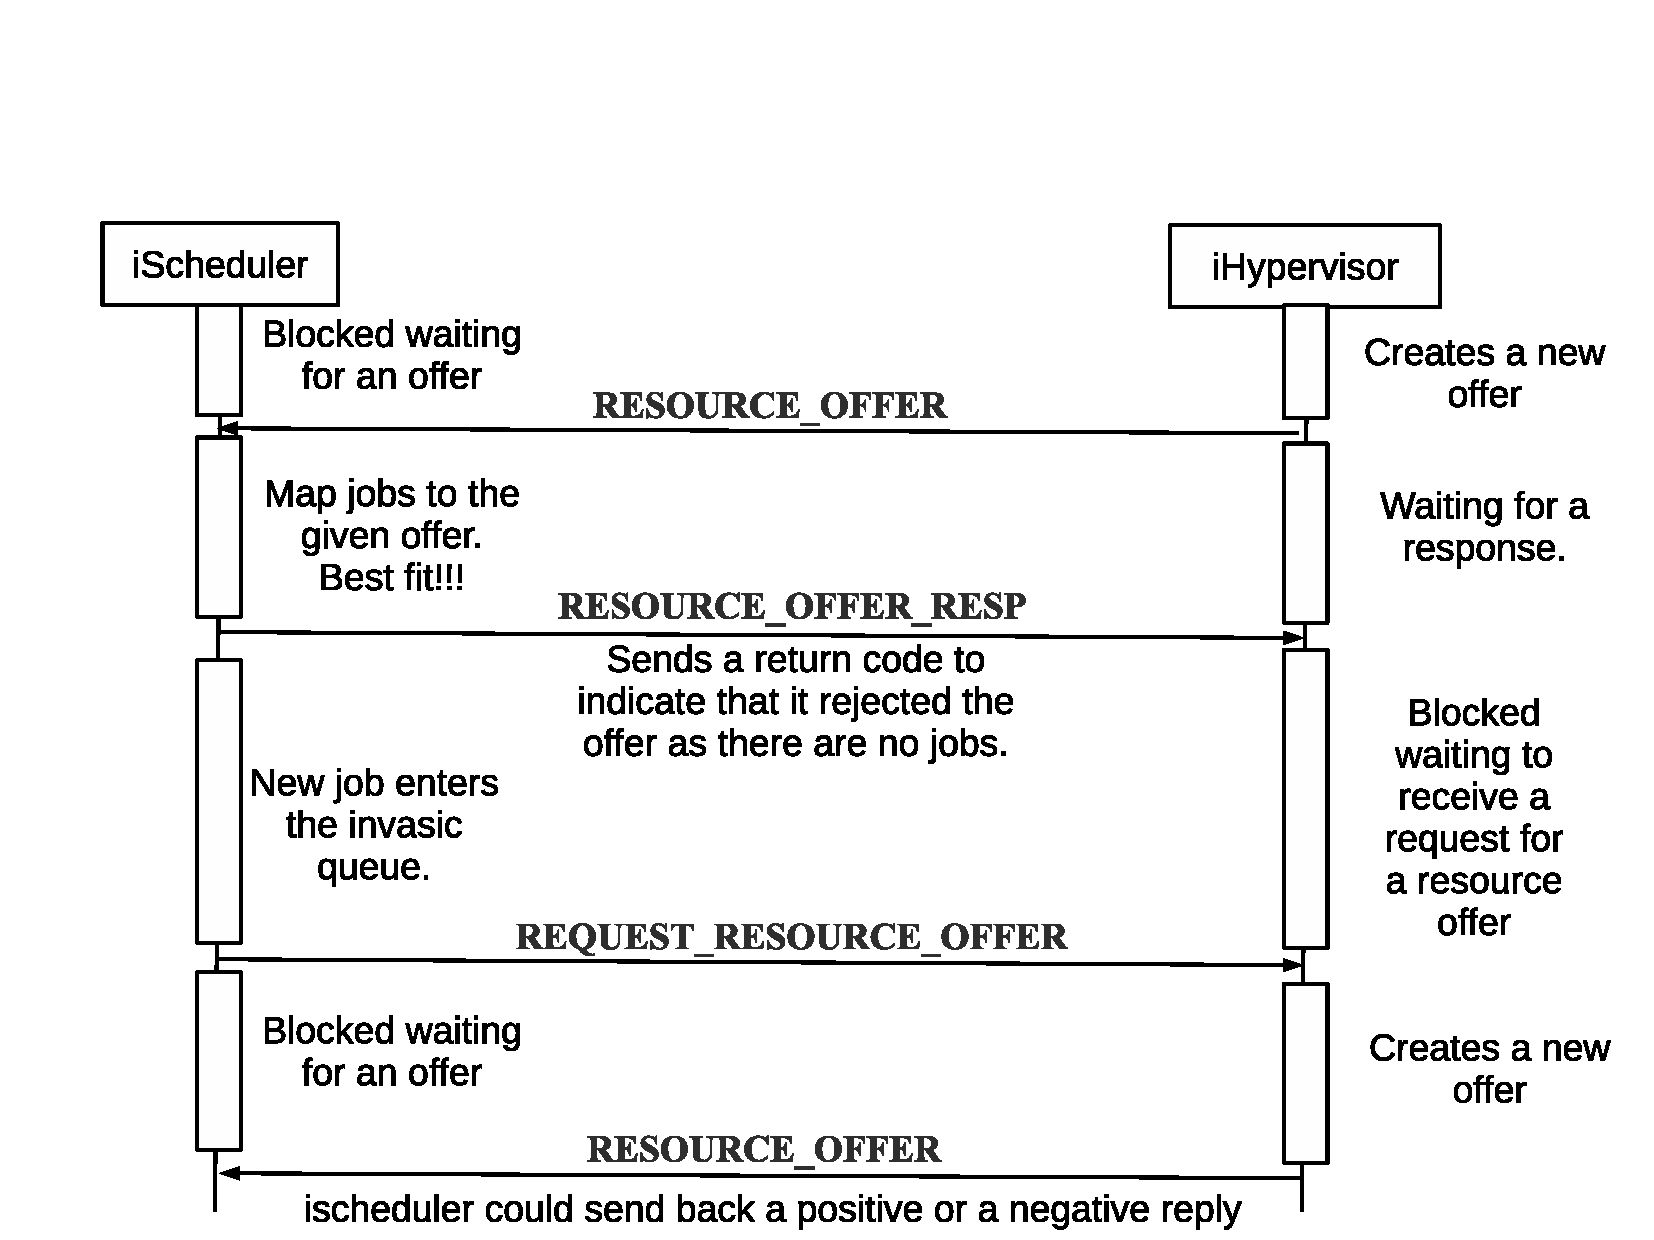
\includegraphics[width=0.9\textwidth, height=100mm]{./figures/figures2.pdf}
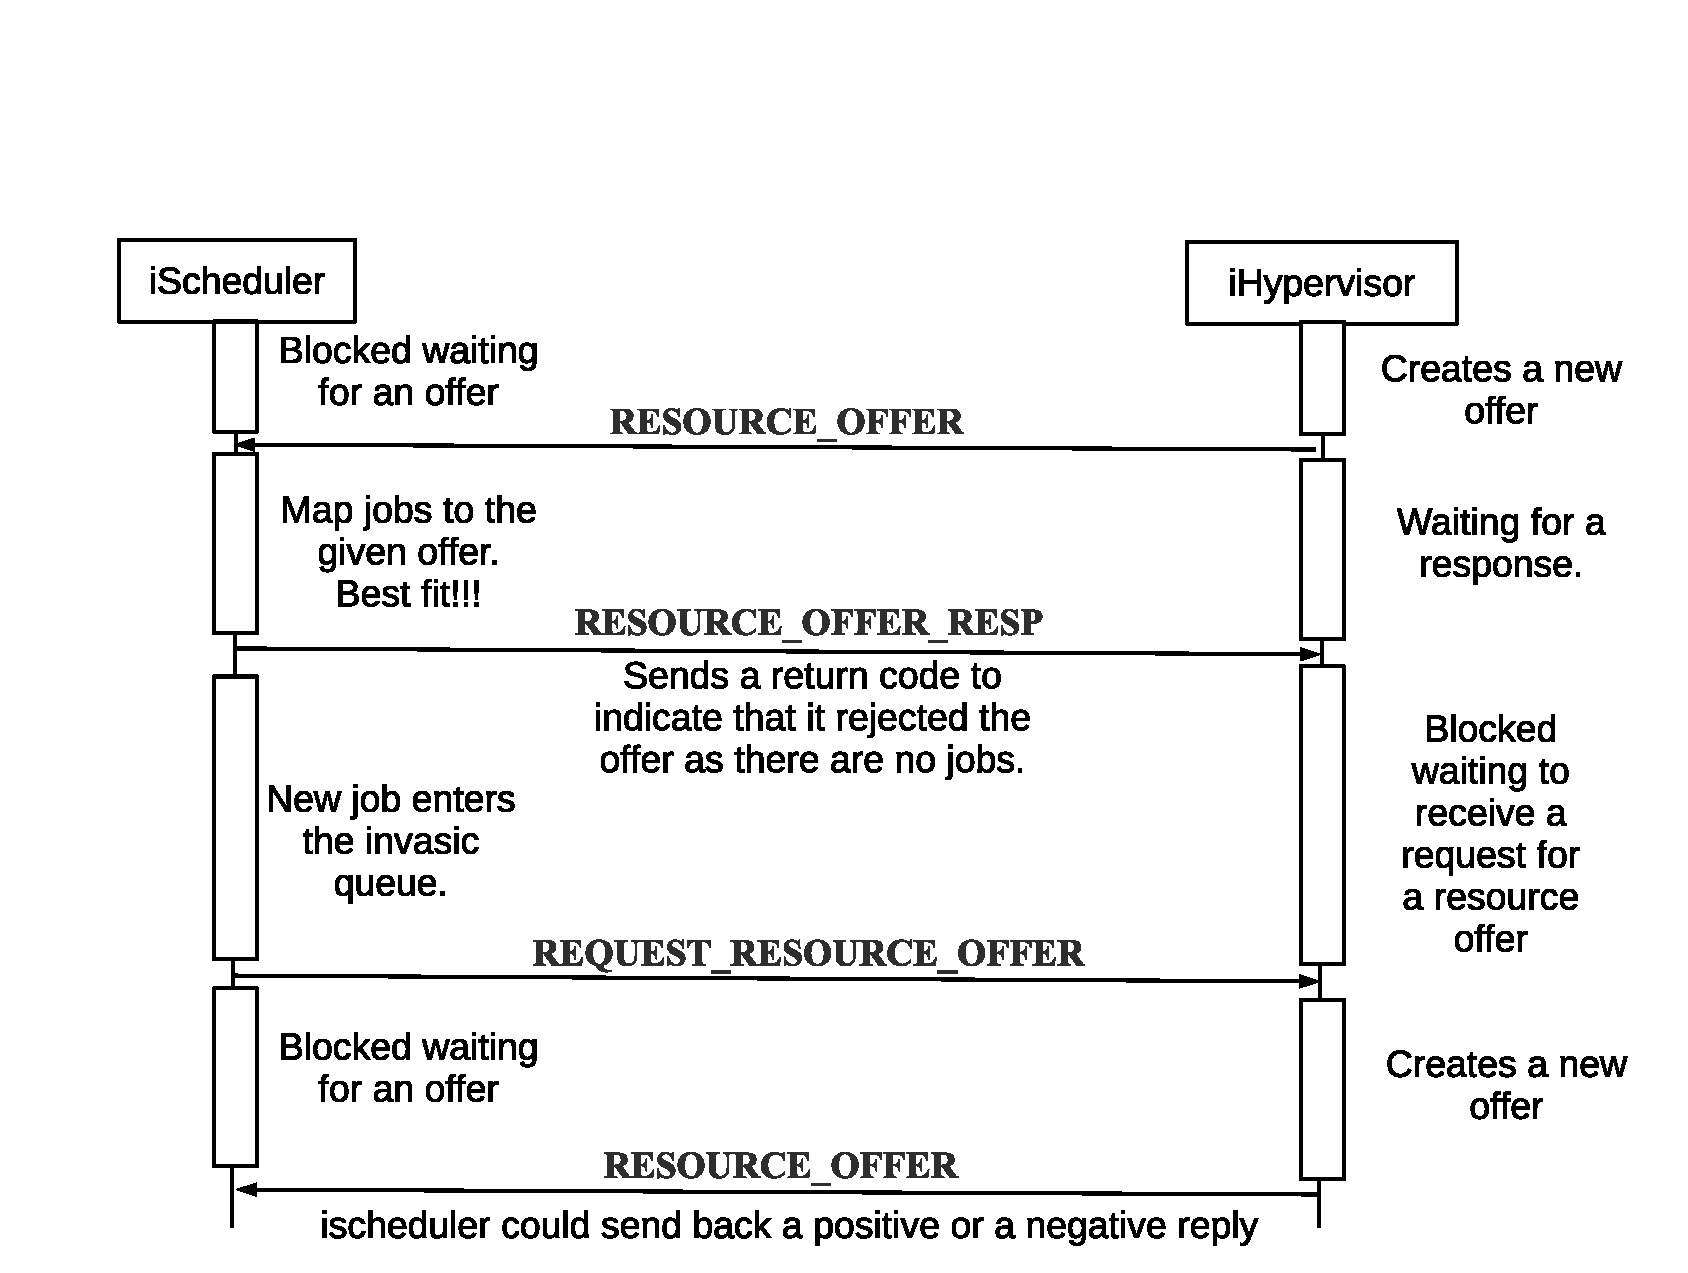
\includegraphics[width=0.9\textwidth, height=100mm]{./figures/figures2.eps}
\caption{Scenario 2}
\label{fig:Seq2}
\end{figure}
\subsection{State Machine Diagrams}
This section focuses on iScheduler and a thread iRM\_AGENT that it spawns which is the one responsible for all the communication with the iHypervisor including spawning other agent threads for handling feedbacks and urgent jobs.
\vspace{10mm}
\begin{figure}[h]
\centering
%\includegraphics[width=1.0\textwidth, height=150mm]{./figures/"iRM Agent".pdf}
\includegraphics[width=1.0\textwidth, height=150mm]{./figures/"iRM Agent".eps}
\caption{iRM Agent}
\label{fig:Init}
\end{figure}
\begin{itemize}
\item Above diagram and the ones in the following pages illustrate state machine diagrams for few of the communication phases described earlier starting first with a general diagram of how the mulithreaded component iRM agent inside iScheduler starts up and shuts down.
\end{itemize}
\vspace{-20mm}
\begin{figure}[h]
\centering
%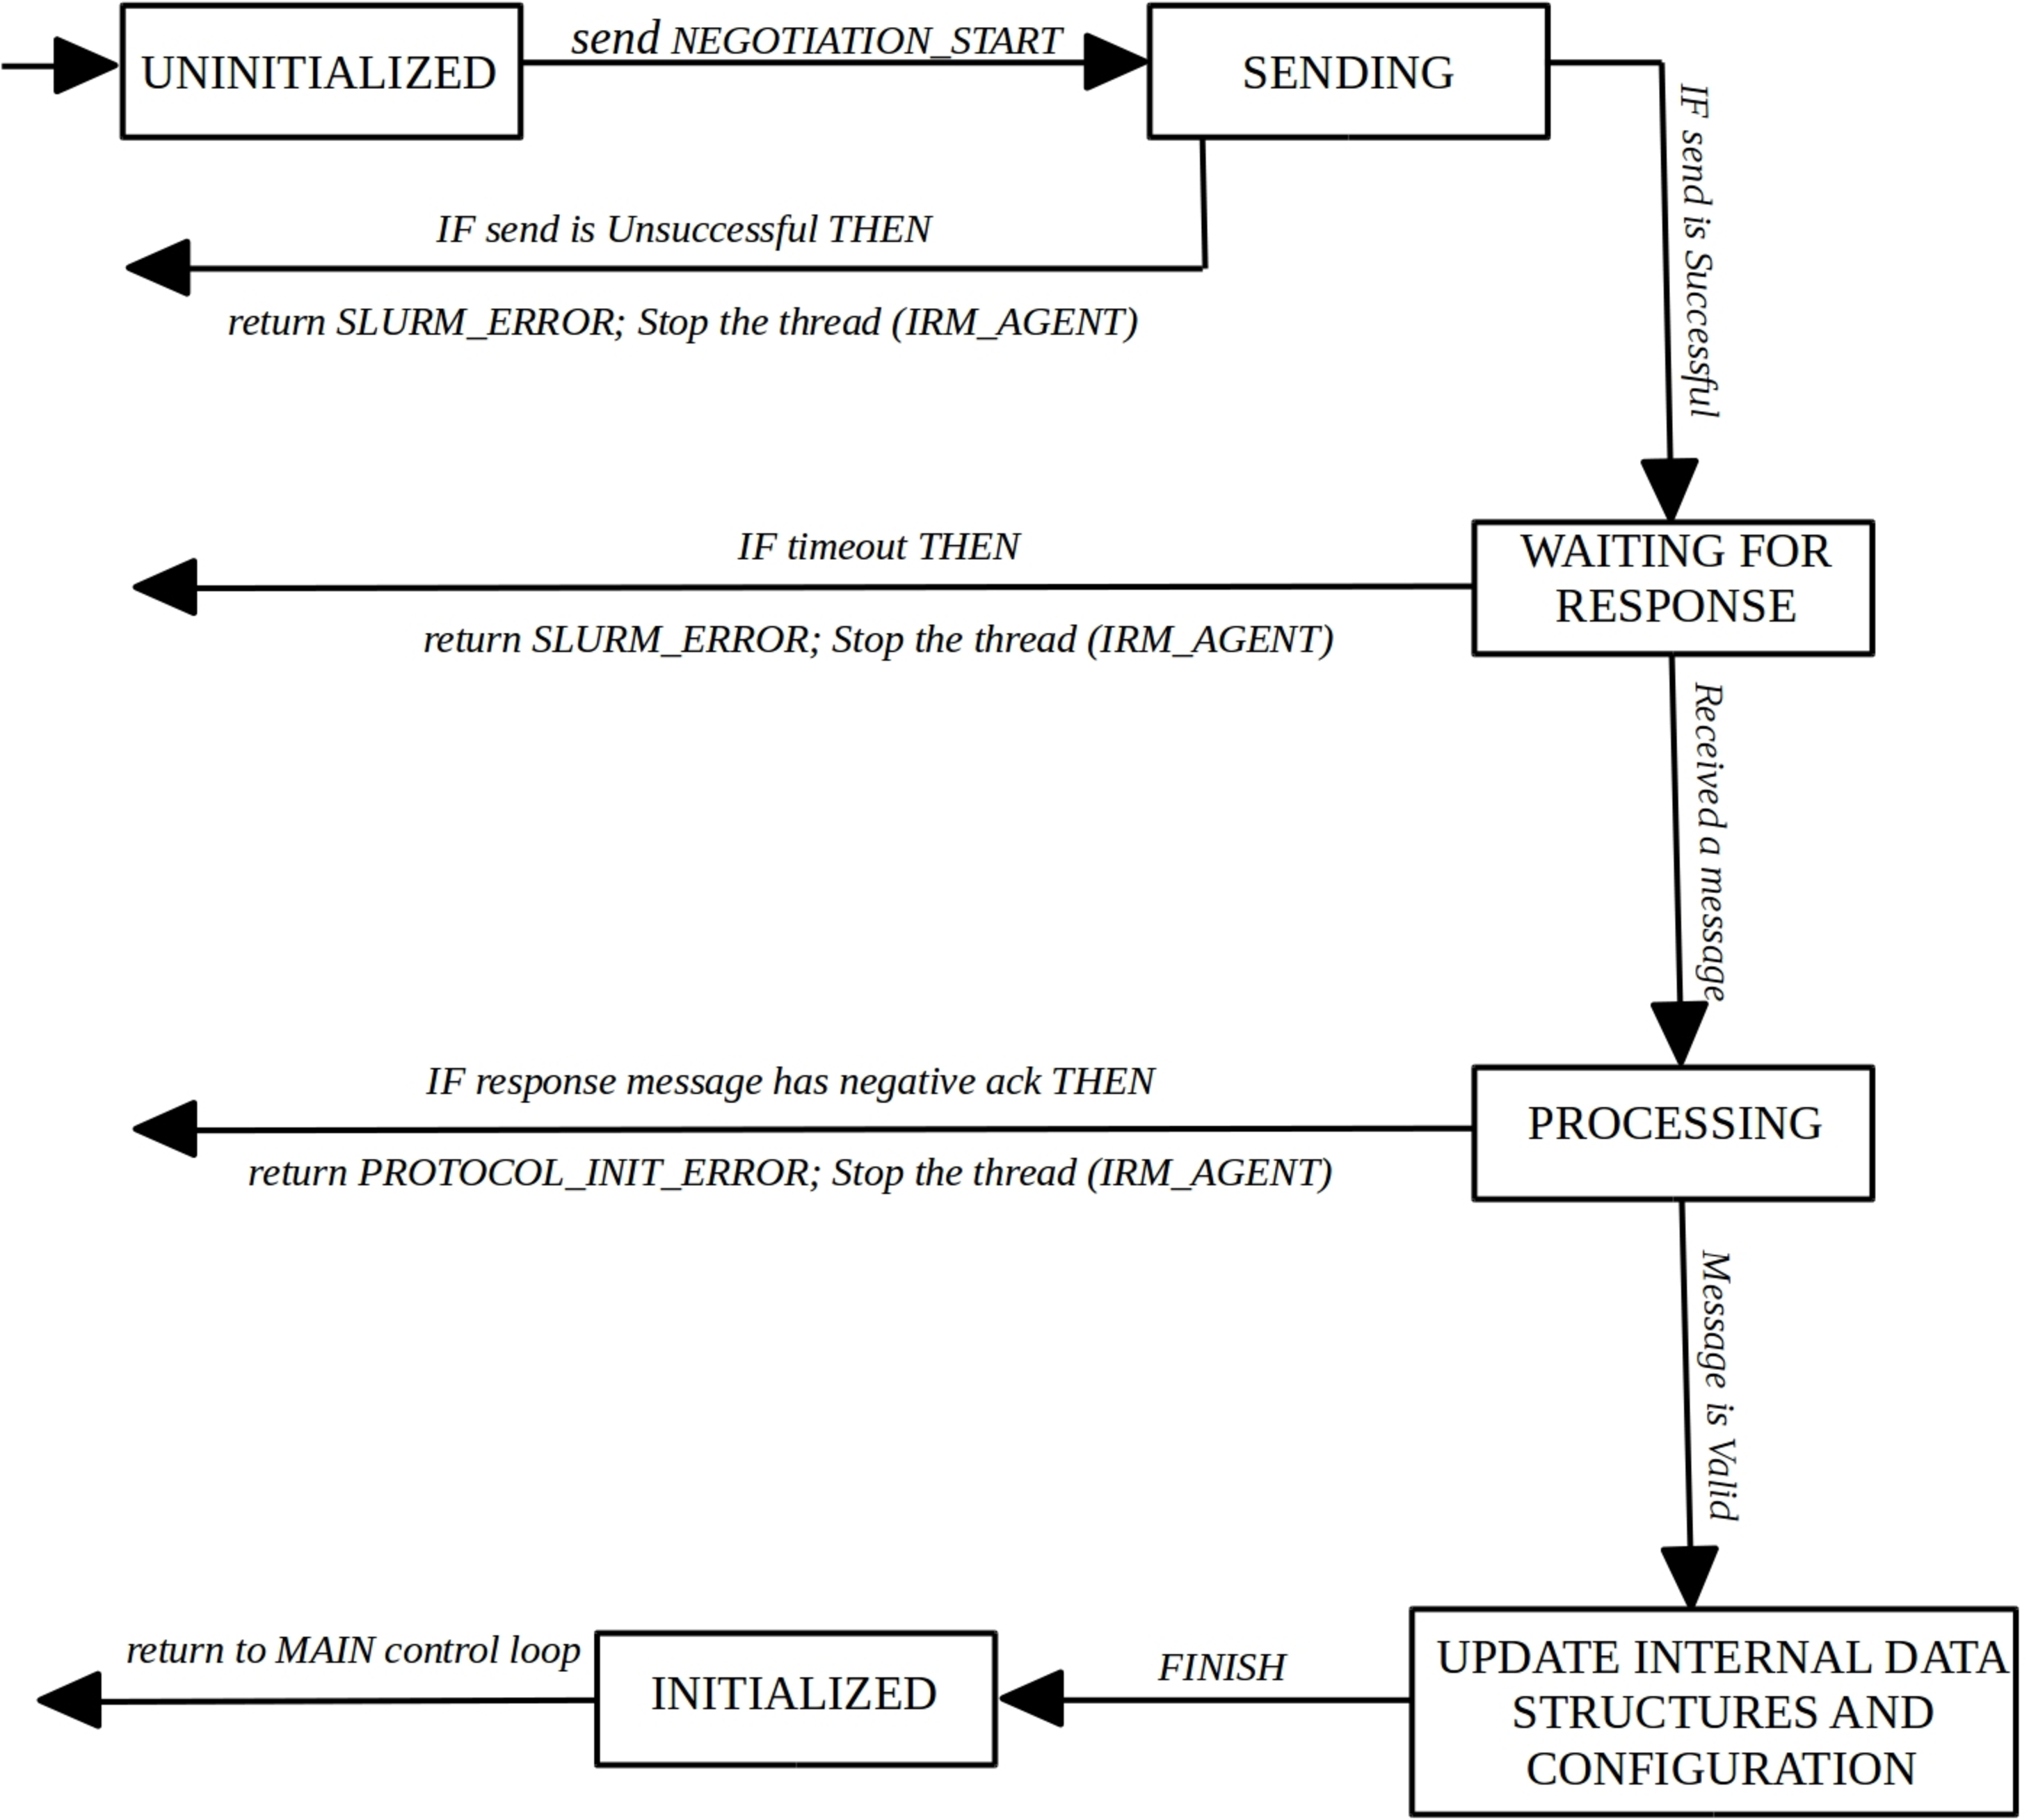
\includegraphics[width=0.9\textwidth, height=90mm]{./figures/Init.pdf}
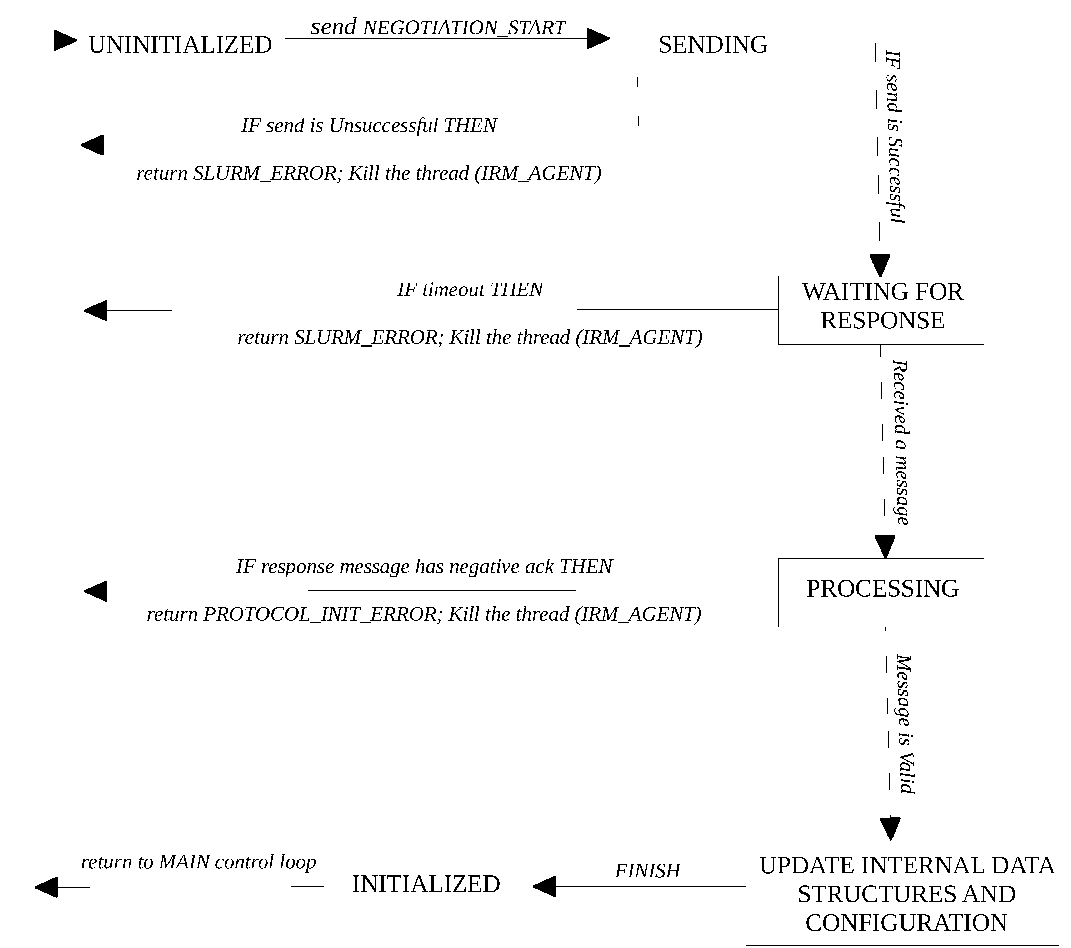
\includegraphics[width=0.9\textwidth, height=90mm]{./figures/Init.eps}
\caption{Protocol Initialization}
\label{fig:Init}
\end{figure}
\vspace{5mm}
\begin{figure}[h]
\centering
%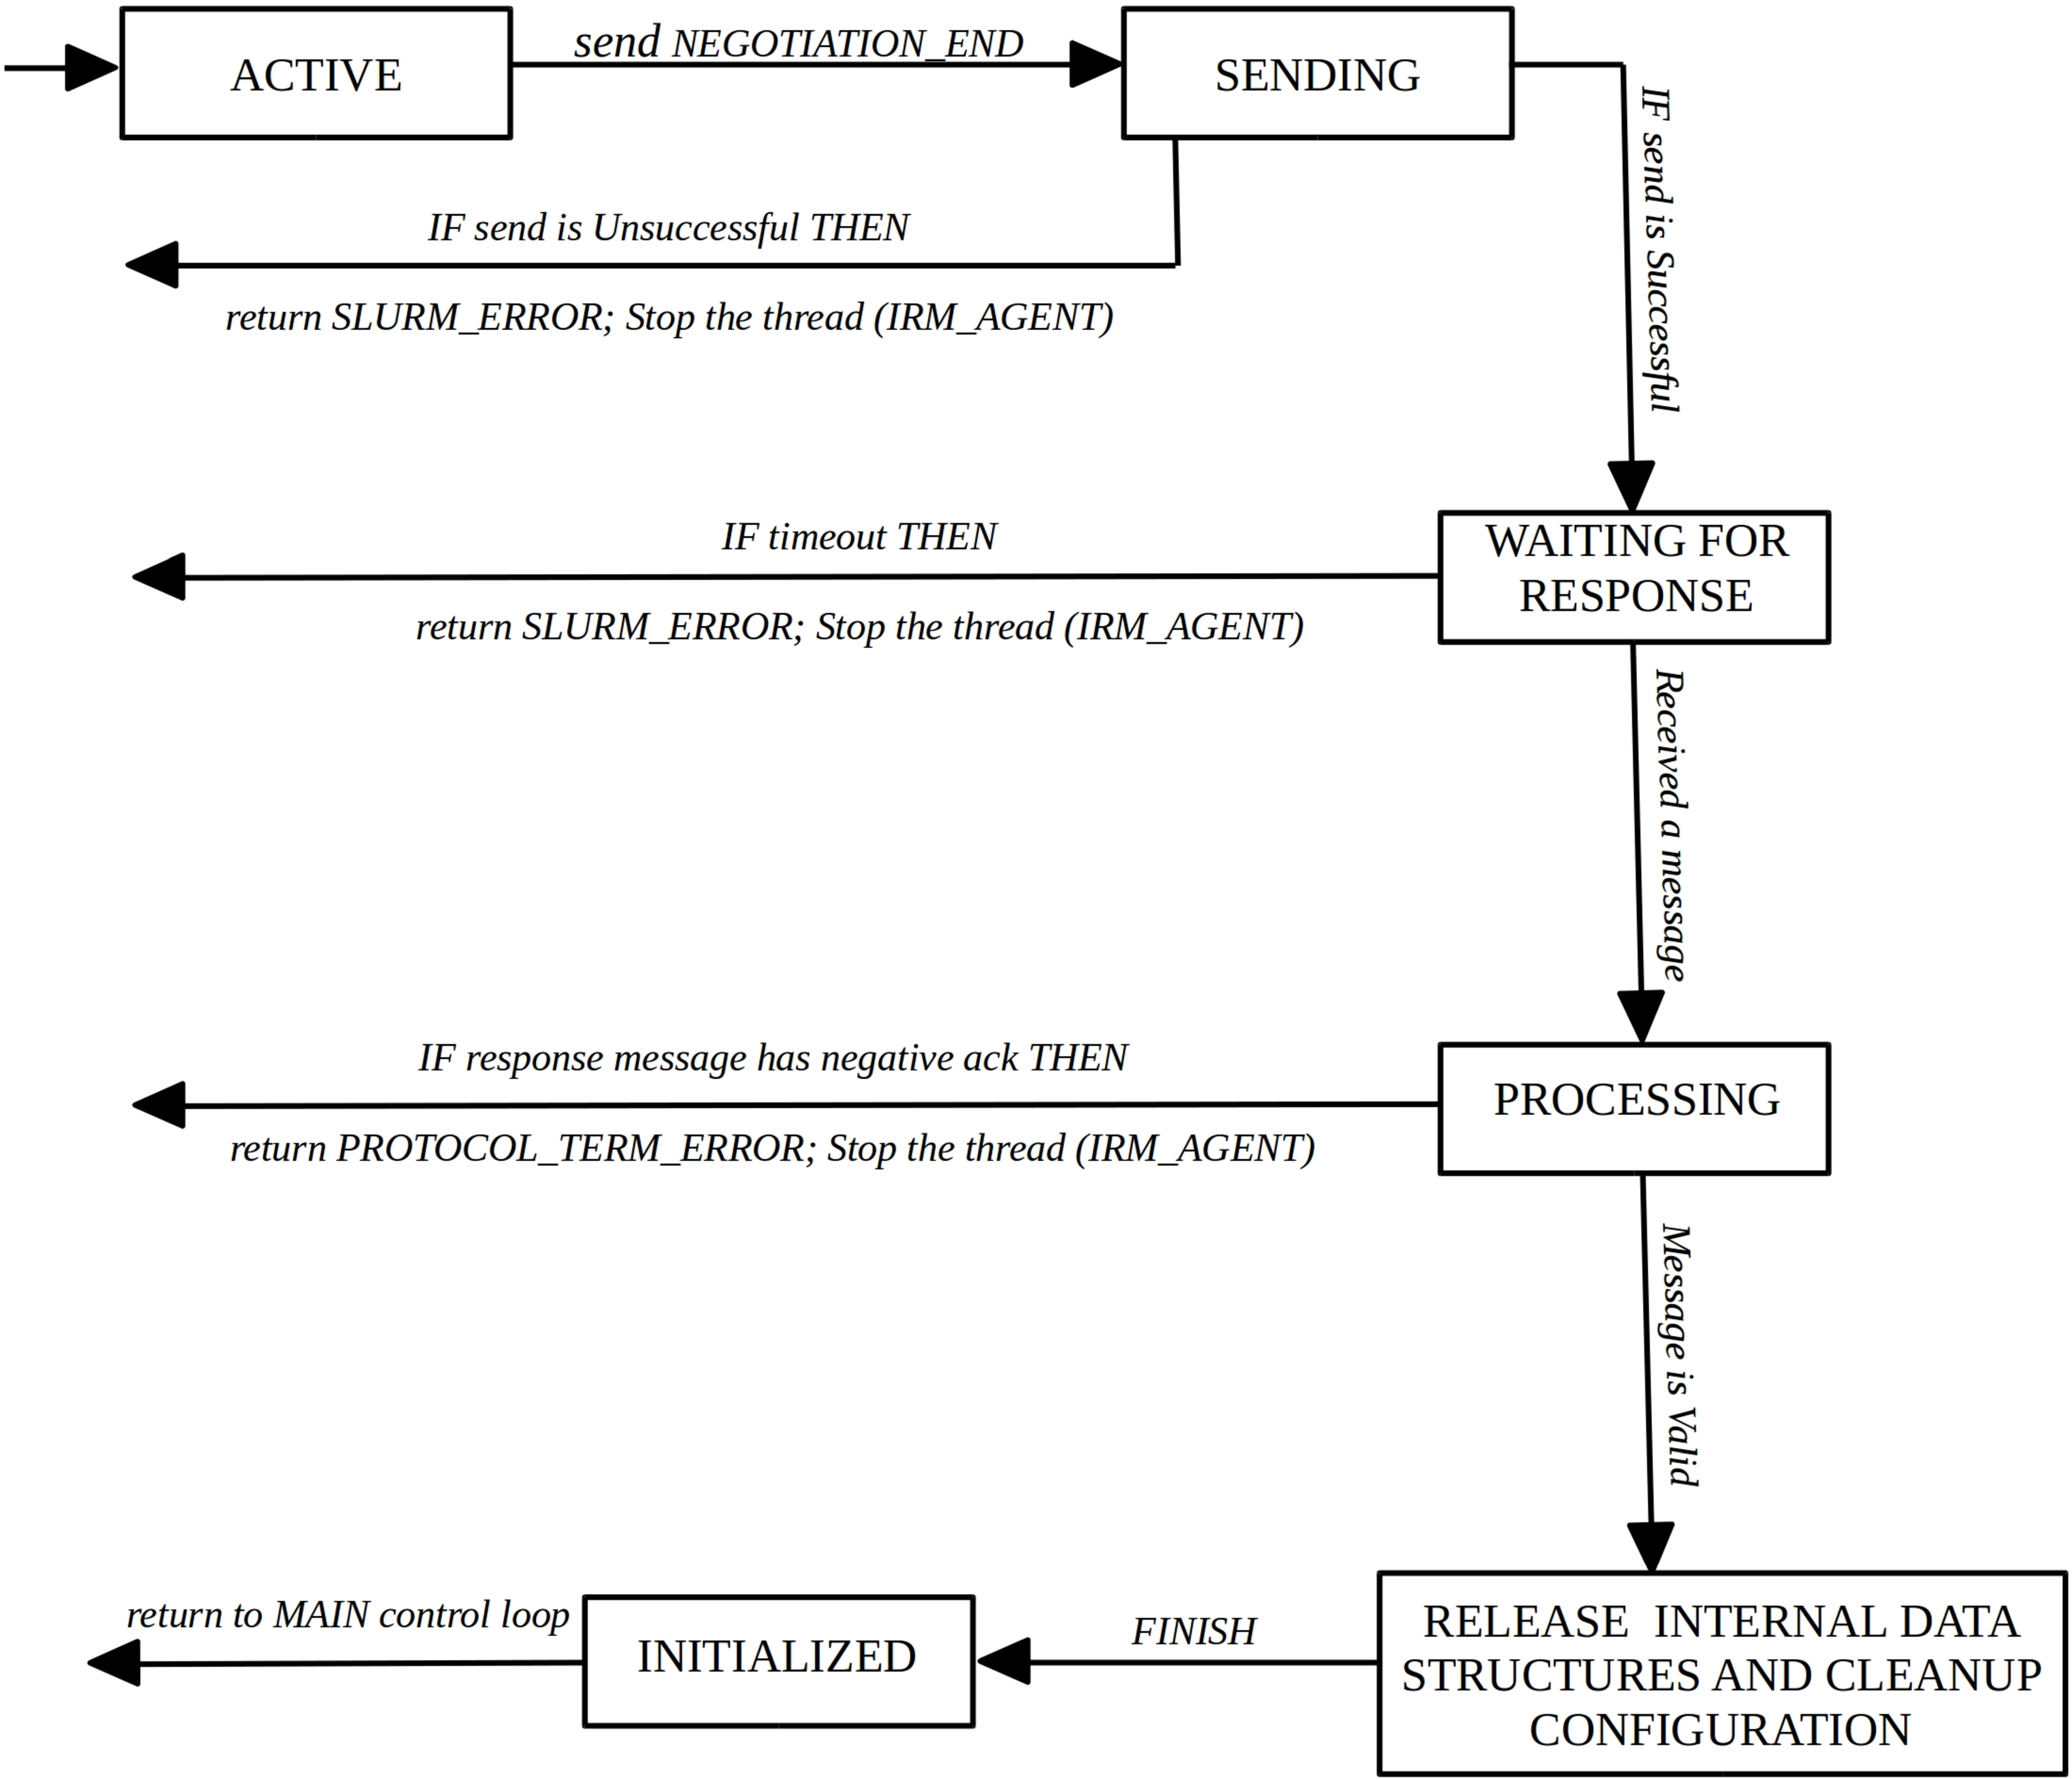
\includegraphics[width=0.9\textwidth, height=90mm]{./figures/Term.pdf}
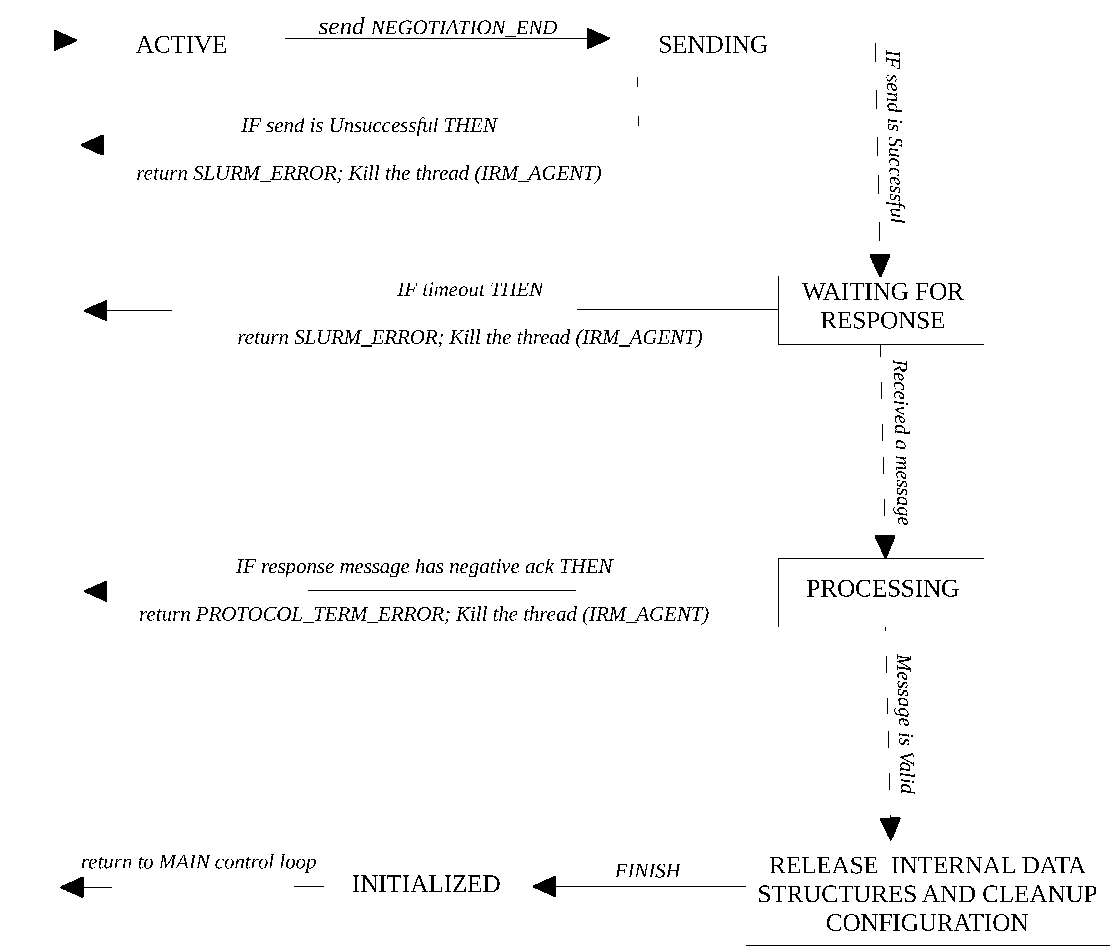
\includegraphics[width=0.9\textwidth, height=90mm]{./figures/Term.eps}
\caption{Protocol Termination}
\label{fig:Term}
\end{figure}
\clearpage
\begin{figure}[h]
\centering
%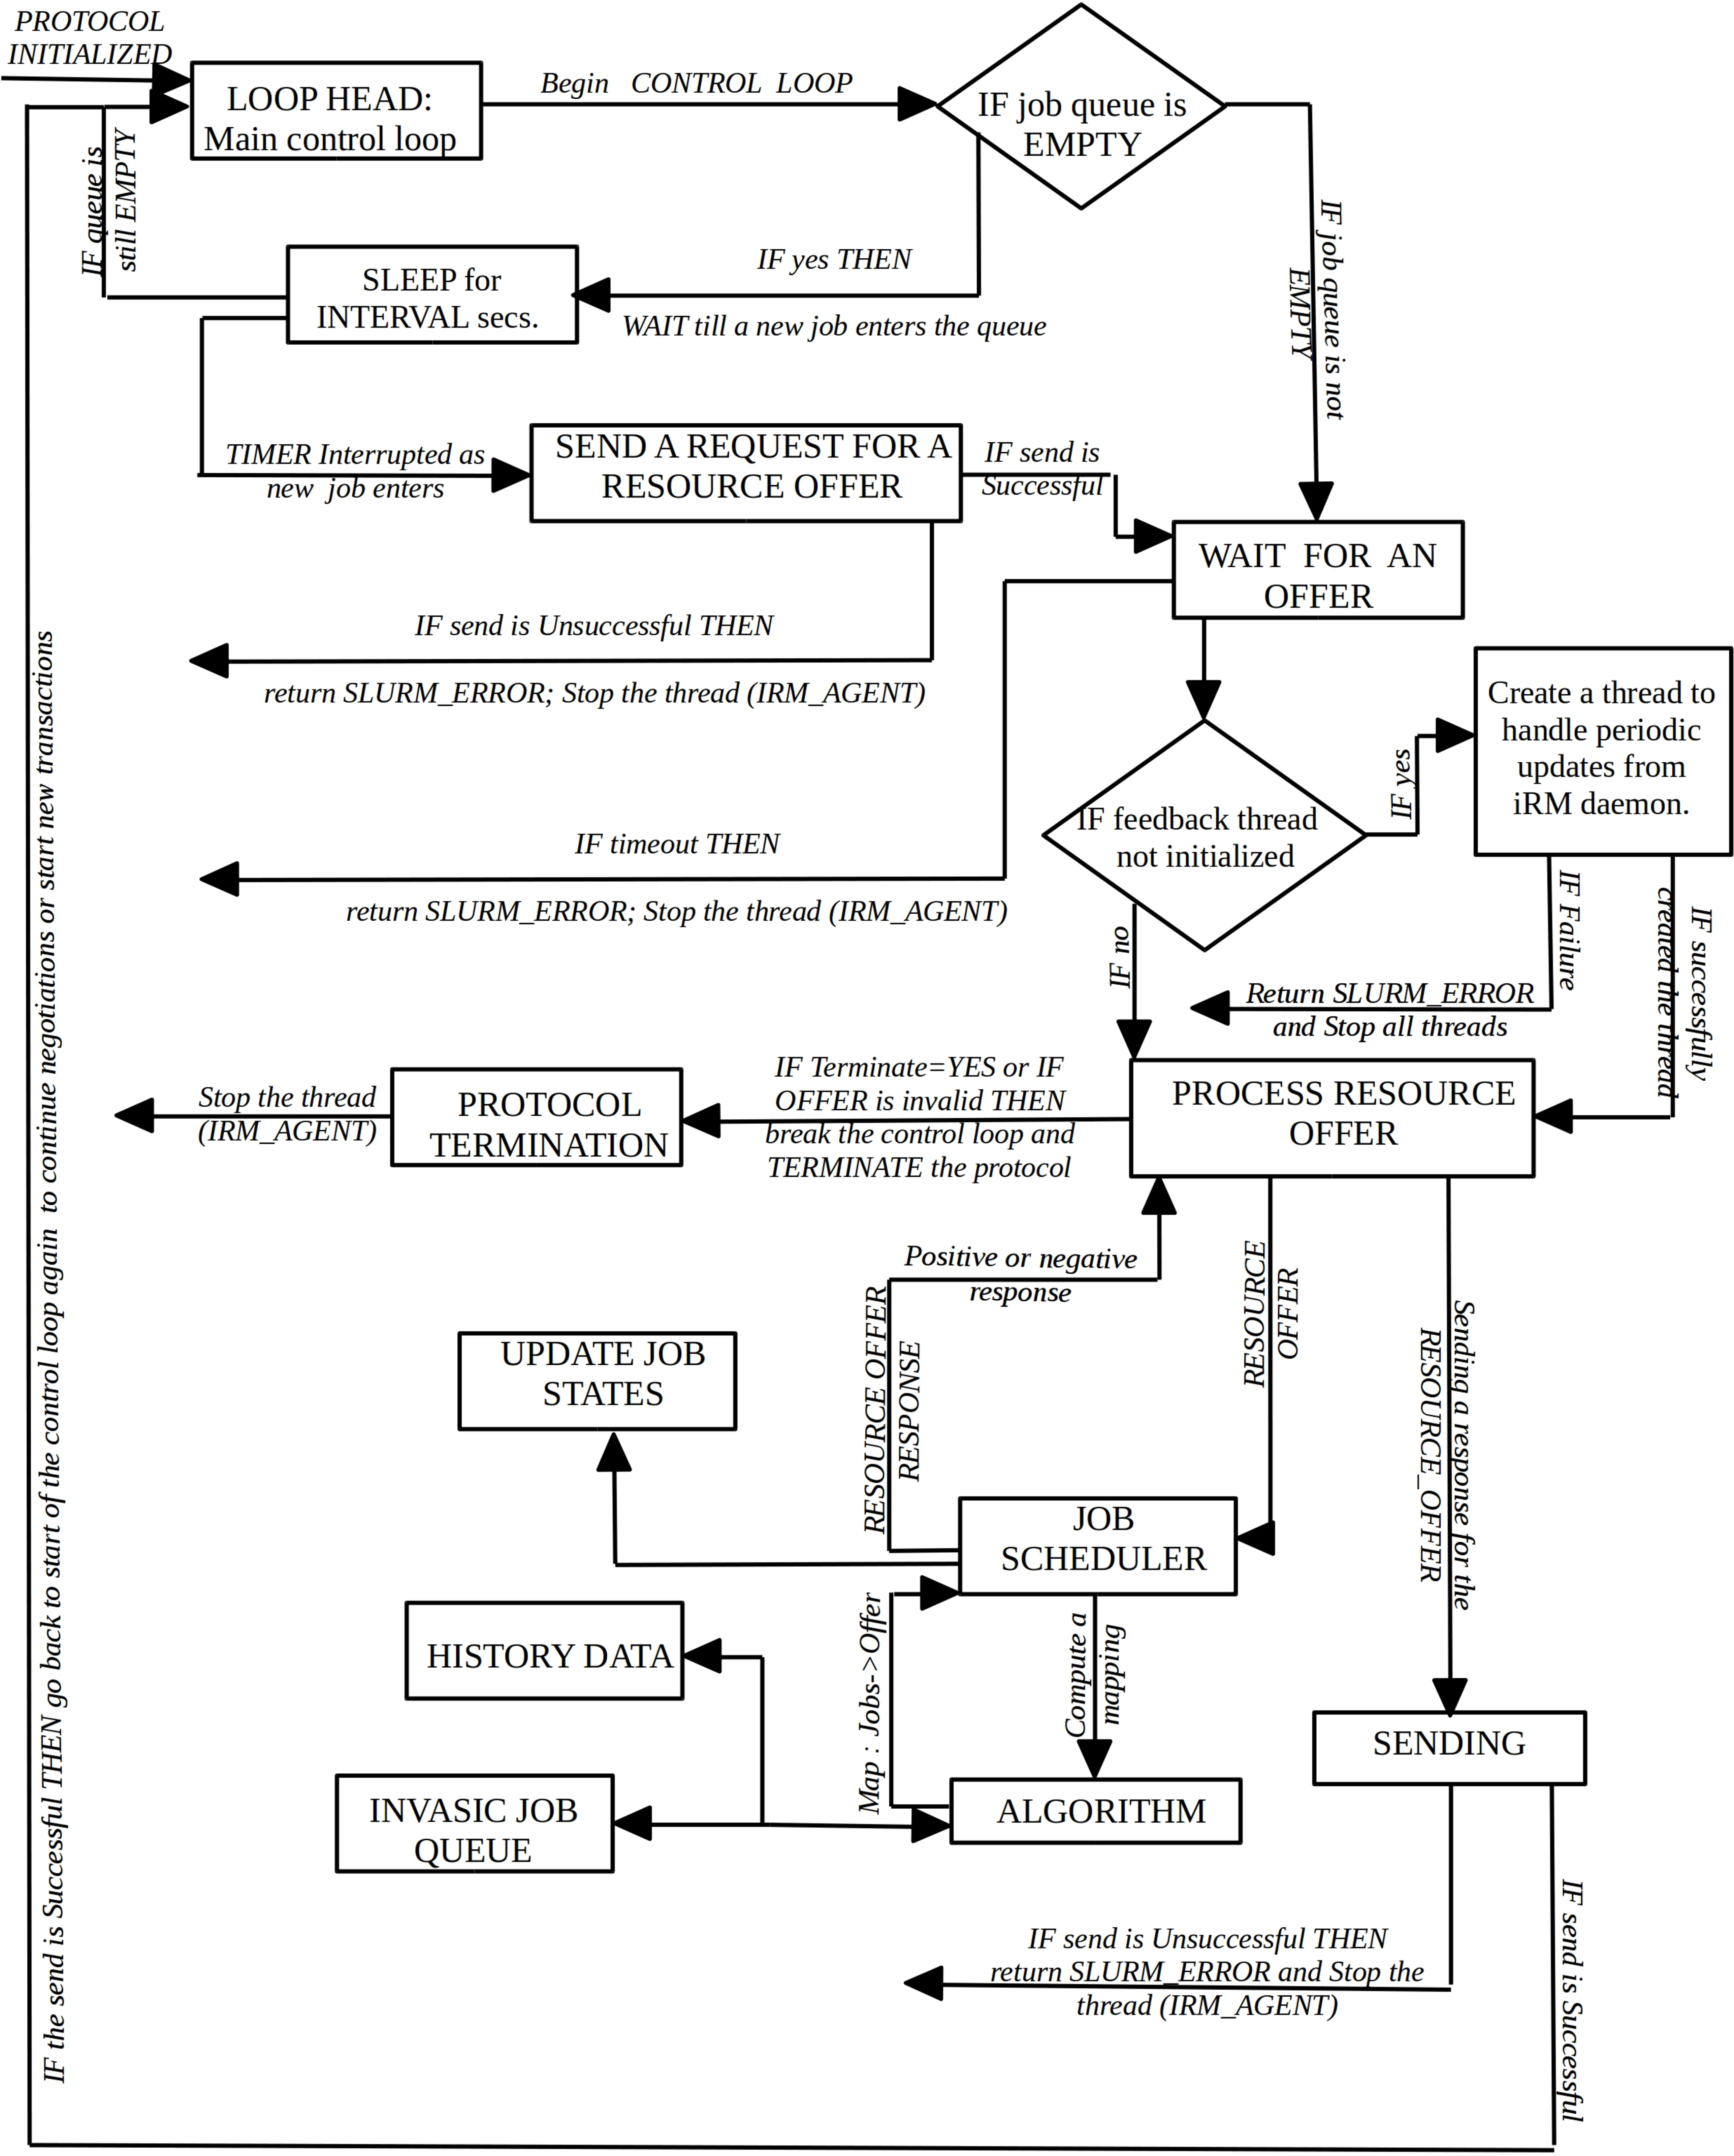
\includegraphics[width=1.0\textwidth, height=210mm]{./figures/Negotiation.pdf}
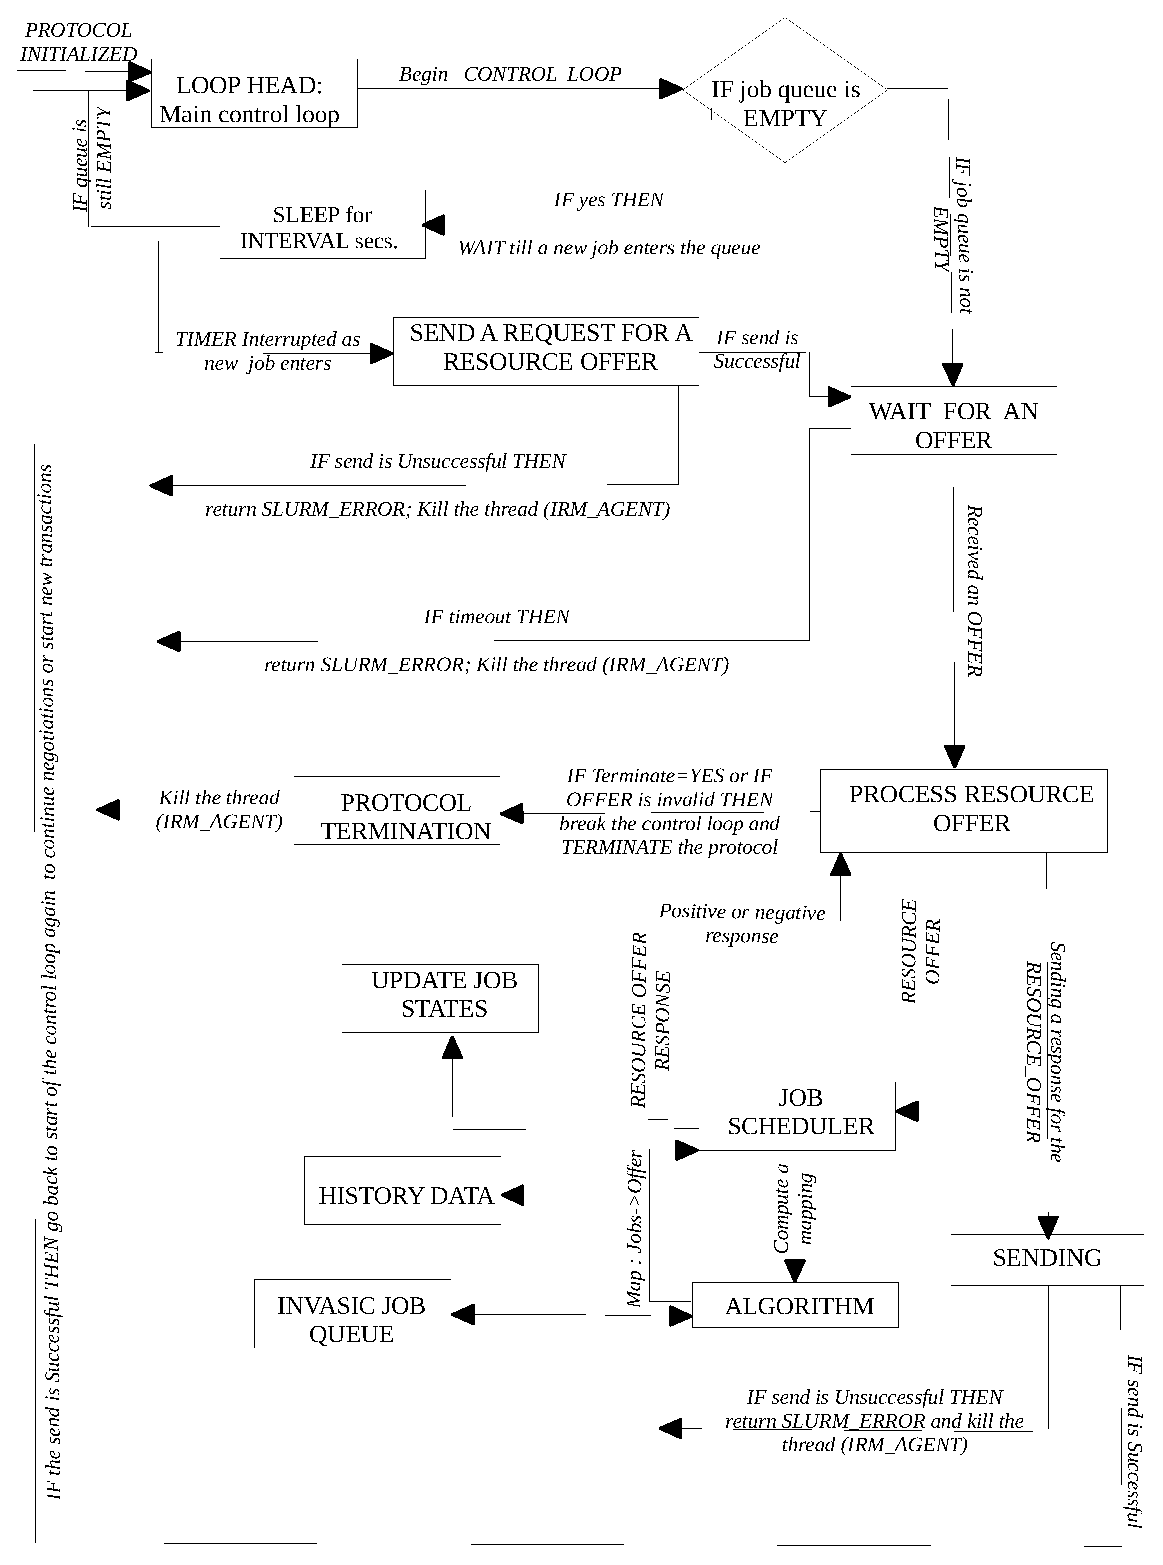
\includegraphics[width=1.0\textwidth, height=210mm]{./figures/Negotiation.eps}
\caption{Negotiation}
\label{fig:Neg}
\end{figure}
\clearpage

\section{Invasive Jobs}
